% Autor: Leonhard Segger, Alexander Neuwirth
% Datum: 2017-10-30
\documentclass[
	% Papierformat
	a4paper,
	% Schriftgröße (beliebige Größen mit „fontsize=Xpt“)
	12pt,
	% Schreibt die Papiergröße korrekt ins Ausgabedokument
	pagesize,
	% Sprache für z.B. Babel
	ngerman
]{scrartcl}

% Achtung: Die Reihenfolge der Pakete kann (leider) wichtig sein!
% Insbesondere sollten (so wie hier) babel, fontenc und inputenc (in dieser
% Reihenfolge) als Erstes und hyperref und cleveref (Reihenfolge auch hier
% beachten) als Letztes geladen werden!

\usepackage{tikz}
\usetikzlibrary{calc,patterns,angles,quotes} % loads some tikz extensions\usepackage{tikz}
\usetikzlibrary{babel}

% Silbentrennung etc.; Sprache wird durch Option bei \documentclass festgelegt
\usepackage{babel}
% Verwendung der Zeichentabelle T1 (Sonderzeichen etc.)
\usepackage[T1]{fontenc}
% Legt die Zeichenkodierung der Eingabedatei fest, z.B. UTF-8
\usepackage[utf8]{inputenc}
% Schriftart
\usepackage{lmodern}
% Zusätzliche Sonderzeichen
\usepackage{textcomp}

% Mathepaket (intlimits: Grenzen über/unter Integralzeichen)
\usepackage[intlimits]{amsmath}
% Ermöglicht die Nutzung von \SI{Zahl}{Einheit} u.a.
\usepackage{siunitx}
% Zum flexiblen Einbinden von Grafiken (\includegraphics)
\usepackage{graphicx}
% Abbildungen im Fließtext
\usepackage{wrapfig}
% Abbildungen nebeneinander (subfigure, subtable)
\usepackage{subcaption}
% Funktionen für Anführungszeichen
\usepackage{csquotes}
\MakeOuterQuote{"}
% Zitieren, Bibliographie
\usepackage{biblatex}
% Zur Darstellung von Webadressen
\usepackage{url}
%chemische Formeln
\usepackage[version=4]{mhchem}
% siunitx: Deutsche Ausgabe, Messfehler getrennt mit ± ausgeben
\usepackage{floatrow}
\floatsetup[table]{capposition=top}
\usepackage{float}
% Verlinkt Textstellen im PDF-Dokument
\usepackage[unicode]{hyperref}
% "Schlaue" Referenzen (nach hyperref laden!)
\usepackage{cleveref}
\sisetup{
	locale=DE,
	separate-uncertainty
}
%\bibliography{14Mo_O4_25-06-2018_References}
%TODO anpassen

\begin{document}
	
	\begin{titlepage}
		\centering
		{\scshape\LARGE Versuchsbericht zu \par}
		\vspace{1cm}
		{\scshape\huge O4 - Magneto-Optischer Kerr-Effekt \par}
		\vspace{2.5cm}
		{\LARGE Gruppe 14Mo \par}
		\vspace{0.5cm}
		
		{\large Alexander Neuwirth (E-Mail: a\_neuw01@wwu.de) \par}
		{\large Leonhard Segger (E-Mail: l\_segg03@uni-muenster.de) \par}
		\vfill
		
		durchgeführt am 25.06.2018\par
		betreut von\par
		{\large Marcel Holtmann} %TODO Überprüfen
		
		\vfill
		
		{\large \today\par}
	\end{titlepage}
	\tableofcontents
	\newpage

	%TODO mehr TODO in Default	

	\section{Kurzfassung}
	%TODO Hypothese	und deren Ergebnis, wenn Hypothese ist, dass nur Theorie erfüllt, sagen: Erwartung: Theorie aus einführung (mit reflink) erfüllt
	%TODO Ergebnisse, auch Zahlen, mindestens wenn's halbwegs Sinn ergibt
	%TODO Was wurde gemacht
	%TODO manche leute wollen Passiv oder "man", manche nicht
	
	\section{Methoden}
	%TODO ziemlich kurz, aber gibt nicht viel mehr zu sagen
	%TODO Temperatur ist relevant.
	In \cref{fig_aufbau} ist der Versuchsaufbau dargestellt.
	Dabei befindet sich eine Probe aus einem Cobalt/Platin-Schichtsystem in einem Magnetfeld, das von zwei Spulen zwischen zwei Polschuhen aufgebaut wird.
	Zunächst wird das Magnetfeld am Ort der Probe in Abhängigkeit vom durch die Spulen fließenden Strom gemessen, indem anstelle der Probe eine Hallsonde zwischen die Polschuhe gebracht wird.
	Diese wird in einem Winkel von ca. \SI{45}{\degree} zur Strecke, die die Polschuhe verbindet, positioniert, da eine Messung in Magnetfeldrichtung aufgrund der Polschuhe nicht möglich ist.
	Dazu wird der Strom von \SIrange{0}{1}{\ampere} in \SI{0,05}{\ampere} Schritten erhöht.
	Dies wird dann bei umgekehrter Flussrichtung wiederholt.

	Dann wird die Probe zwischen die Polschuhe gebracht und ein Laser durch einen Polarisationsfilter als Polarisator auf die Probe gerichtet.
	Ein weiterer Polarisationsfilter wird als Analysator mit einem Polarisationswinkel von \SI{45}{\degree} zum Polarisator in den reflektierten Strahl gebracht, weil gemäß dem Gesetz von Malus die Intensität proportional zum quadrierten Kosinus des Differenz der Polarisationswinkel ist und die Ableitung des quadrierten Kosinus bei einem Winkel von \SI{45}{\degree} maximal ist.
	Dies führt zu maximaler Messgenauigkeit. %TODO true genug, präzise genug? KP
	Ein Lichtsensor wird so aufgestellt, dass der Strahl in ihm endet.
	
	Die vom Lichtsensor gemessene Intensität wird in Abhängigkeit vom Spulenstrom aufgenommen.
	Dabei ist der Raum durch einen Vorhang abgedunkelt und der Strom wird wie zuvor in beiden Flussrichtungen schrittweise erhöht.
	
	\begin{figure}[H] 
		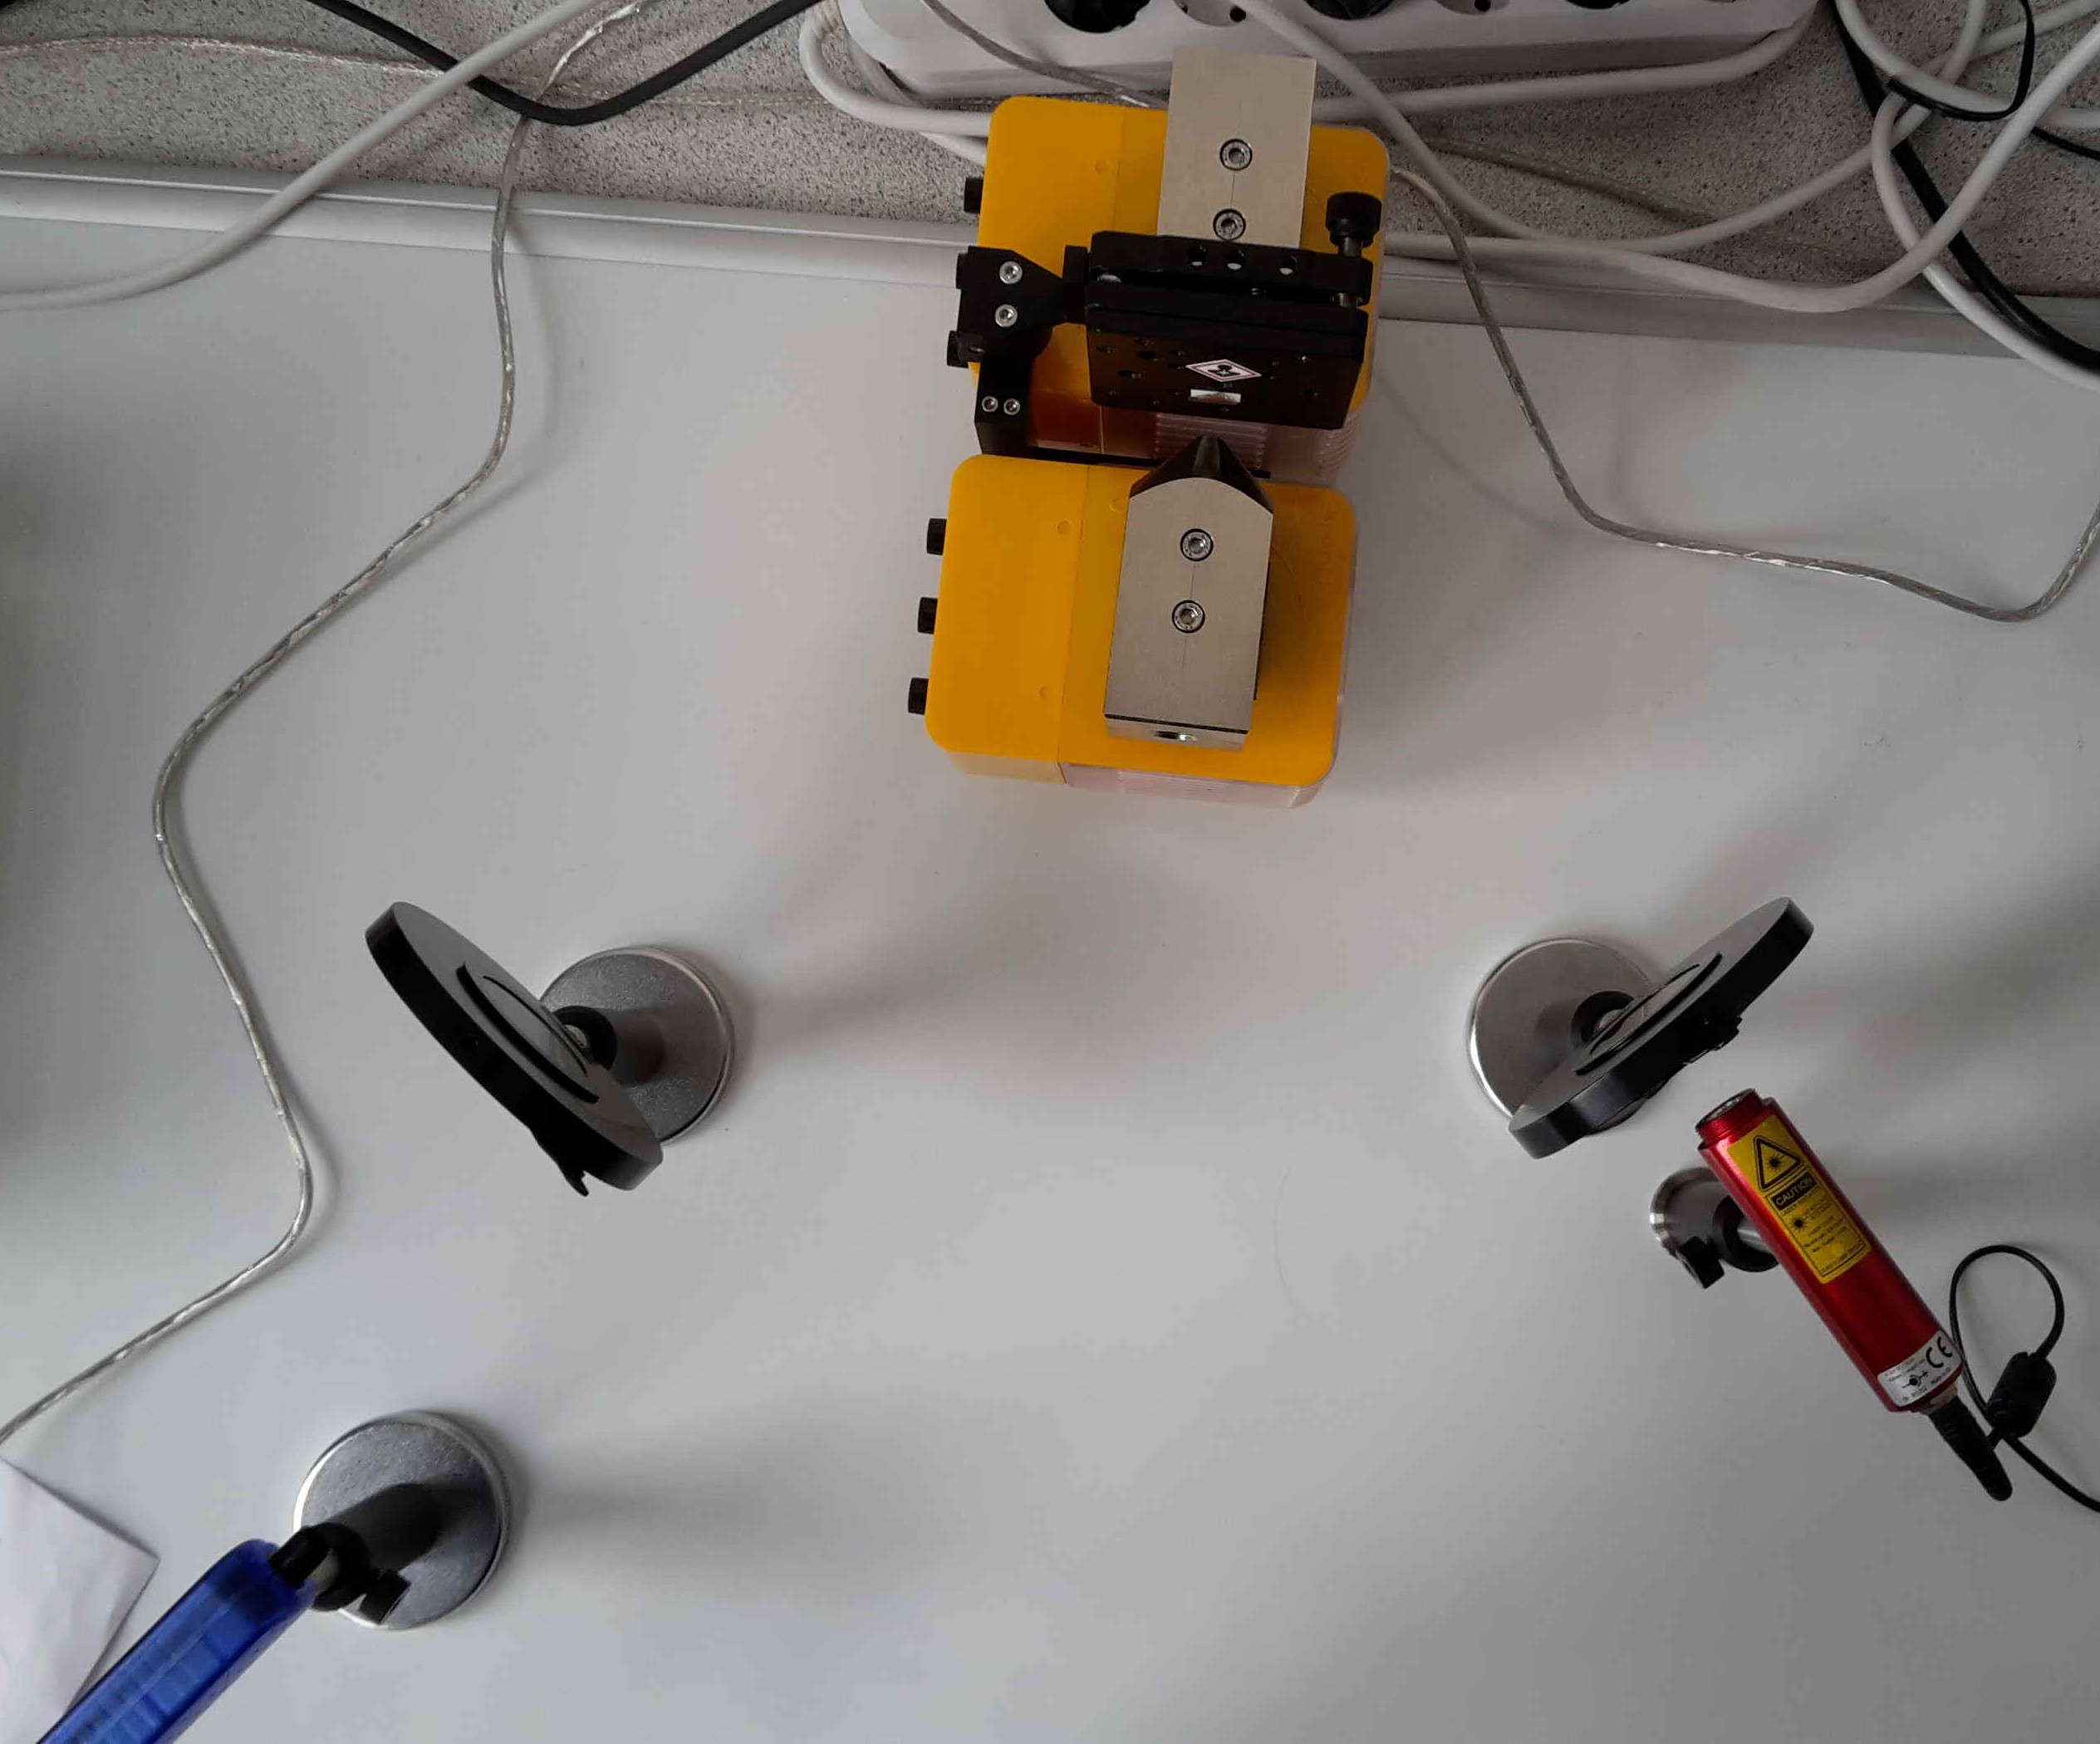
\includegraphics[width=0.7\textwidth]{O4_Aufbau} %TODO größe anpassen am Ende
		\centering
		\caption{Elemente des Aufbaus des Experiments. Ein linear polarisierter Laserstrahl trifft auf eine Probe aus einem Cobalt/Platin-Schichtsystem, die sich in einem Magnetfeld befindet. Der reflektierte Strahl trifft durch einen Polarisationsfilter in einen Lichtsensor. Aus Übersichtsgründen sind keine Kabel an die Spulen angeschlossen. Die optischen Komponenten sind im Bild nicht justiert.} 
		\label{fig_aufbau}
		\centering
	\end{figure}
	
	\section{Ergebnisse und Diskussion}
	%TODO Unsicherheiten
	

	\subsection{Beobachtung und Datenanalyse}
	%TODO Einflüsse von veränderten Parametern auf Messung
	\subsubsection{Unsicherheiten} %TODO GGF IN DATENANYLSY
	Die Unsicherheiten werden gemäß GUM ermittelt. 
	Außerdem wird für Unsicherheitsrechnungen die Python-Bibliothek "uncertainties" verwendet.
	\begin{description}
		\item[Amperemeter/Multimeter:] Der Messwert des Betriebsstroms der Spulen wird von einem Multimeter abgelesen. 
			Dieses zeigt die Stromstärke auf zwei Nachkommastellen genau an. 
			Es ergibt sich also eine Unsicherheit von \SI{3}{mA} (rechteckige WDF).
			Dabei wird angenommen, dass der eigentliche Messfehler des Gerätes dem Displayfehler gegenüber verschwindet. 
		\item[Hall-Sonde:]  Die Stärke des Magnetfelds wird mit einer Hall-Sonde gemessen. Die Messwerte schwanken in der fünften Nachkommastelle, sodass eine Unsicherheit von \SI{30}{\mu T} angenommen wird.
		\item[Photodiode:]  Die relative Intensität des Lichts wird mit einer Photodiode gemessen. Die Unsicherheit bei dieser Messung wird mit \SI{0,1}{} abgeschätzt.
	\end{description} 

	\subsubsection{Bestimmung des Magnetfelds}
	Die Stärke des Magnetfelds an der Position der Probe wird mit der Hall-Sonde in einem Winkel $\theta$ gemessen.
	Für ein $\theta=\SI{90}{\degree}$ wurde $\vec B_\text{Mess} = \SI{0,1}{mT}$ gemessen.
	In \cref{fig_draw} sind die Winkelverhältnisse dargestellt. 
	$\vec B$ ist das Magnetfeld senkrecht zur Probenoberfläche. 
	$\vec B_\text{Hall}$ zeigt die Messrichtung der Hall-Sonde an.
	Der Messwert $ \left| \vec B_\text{Mess}\right| $ ist die Projektion von $\vec B$ auf $\vec B_\text{Hall}$:
	\begin{equation}
		\left| \vec B_\text{Mess}\right|  = \vec B \cdot \frac{\vec B_\text{Hall}}{\left| B_\text{Hall} \right|} = \left| B \right| \cdot \cos(\theta)
	\end{equation}
	Mit $\theta=\SI{45\pm 2}{\degree}$ folgt also $B = (\sqrt{2}\pm0,05) \cdot B_\text{Mess}$.

	\begin{figure}[H]
		\centering
		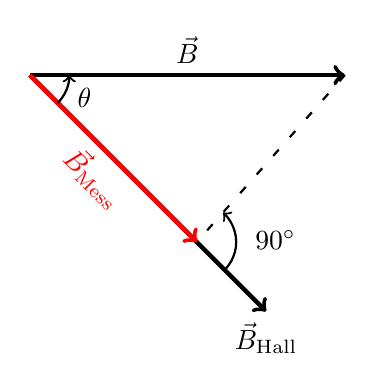
\begin{tikzpicture} %dafuq, ziemlich nice
			\coordinate (ori) at (0,0);
			\coordinate (mag) at (4,0);
			\coordinate (hall) at (3,-3);
			\coordinate (senk) at (2.12,-2.12);

			\draw[->, ultra thick] (ori) -- (mag) node [pos=.5,sloped,above] {$\vec B$};
			\draw[->,ultra thick] (ori) -- (hall) node [sloped,below] {$\vec B_\text{Hall}$};
			\draw[->,ultra thick,color=red] (ori) -- (senk) node [pos=.5,sloped,below] {$\vec B_\text{Mess}$};
			\draw[loosely dashed, thick] (mag) -- (senk) node [pos=.5,sloped,above] {};
			\pic[draw, ->, thick, angle eccentricity=1.5,"$\theta$"] {angle = hall--ori--mag};
			\pic[draw, ->, thick, angle eccentricity=2.0,"$\SI{90}{\degree}$"] {angle = hall--senk--mag};
		\end{tikzpicture}
		\caption{Skizze zur Veranschaulichung der Messung des Magnetfelds in Abhängigkeit vom Stromfluss durch die Spulen.}
		\label{fig_draw}
	\end{figure}
	
	Die Messergebnisse sind in \cref{fig_spule} dargestellt. 
	Da ein linearer Zusammenhang erwartet wird, wird ein linearer Fit berechnet.
	Der y-Achsenabschnitt $b$ ist vernachlässigbar klein, sodass sich als Proportionalitätsfaktor zwischen Stromstärke und B-Feld von $a= \SI{-0,0532+-0,0001}{T/A}$ ergibt.
	\begin{figure}[H] 
		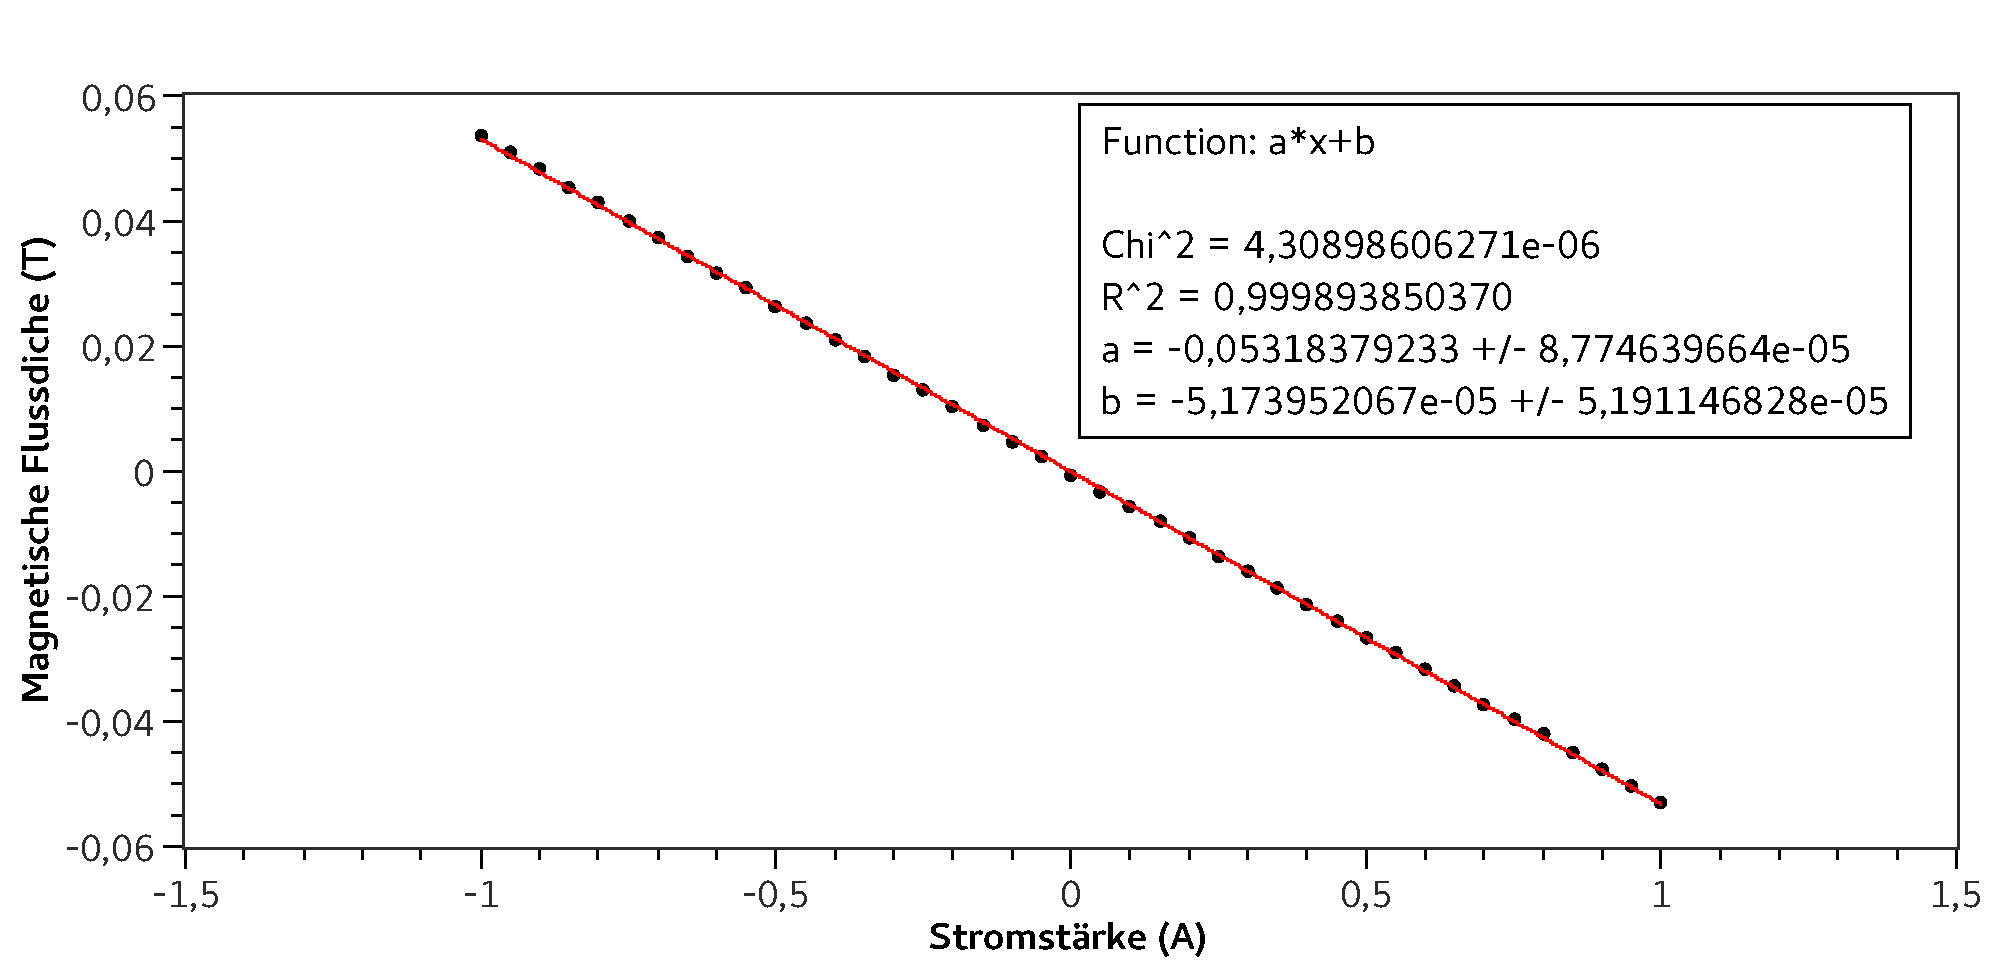
\includegraphics[width=1\textwidth]{fig_spule}
		\centering
		\caption{Die gemessene senkrechte magnetische Flussdichte ist gegen den Betriebsstrom der Spulen aufgetragen. Die Unsicherheiten sind kleiner als die Symbolgröße.} 
		\label{fig_spule}
		\centering
	\end{figure}

	\subsubsection{Messung der Hysterese}
	Aus der Einführung ist bekannt, dass die Lichtintensität proportional zur Magnetisierung ist.
	Die Stärke des magnetischen Felds ergibt sich aus dem in \cref{ss_spule} bestimmten Proportionalitätsfaktor und aus dem Strom, der durch die Spulen fließt.

	Die erste durchgeführte Messung ergab keinen stetigen Verlauf der Magnetisierung. %TODO wie sollen Messpunkte stetig sein? Gib mir besseres Wording anstatt nur zu bemängeln plz, du weißt was gemeint ist.
	Die relative Intensität ist zwischen verschiedenen Werten ohne erkennbaren Bezug zum angelegten Magnetfeld gesprungen.
	Es zeigt sich, dass die Messwerte besser sind, wenn der Raum verdunkelt ist. %TODO besser ist in diesem Zusammenhang nicht wissenschaftlich, ok wie wäre des besser formuliert?
	Des Weiteren wird beobachtet, dass die Messwerte der Photodiode um ca. $\SI{\pm0,2}{}$ schwanken, wenn man an den Tisch stößt.

	Die so gemessene Hystereseschleife ist in \cref{fig_magn1} und \cref{fig_magn2} dargestellt.
	Vor der Messung in \cref{fig_magn1} wird ein negatives Magnetfeld angelegt und dann die Veränderung der Magnetisierung bei steigendem Magnetfeld aufgezeichnet. %TODO negativ ist halt eigentlich willkürlich, aber ich weiß grad auch nicht besser
	Es zeigt sich ein scheinbarer Anstieg der Magnetisierung in einem Bereich von \SI{-0,02+-0,02}{T}. 
	Dieser fällt allerdings wieder auf den bereits bei \SI{-0,055}{T} gemessenen Wert zurück.
	Bei \SI{0,03+-0,001}{T} ist ein deutlicher Sprung in der Magnetisierung zu erkennen und bei noch stärkeren Magnetfeldern scheint sich die Magnetisierung nicht mehr zu ändern.

	Direkt im Anschluss wird die Messung für ein abnehmendes Magnetfeld durchgeführt und in \cref{fig_magn2} dargestellt.
	Nach einem langsam linearen Abnehmen der Magnetisierung zeigt sich ein deutlich steileres Abfallen bei \SI{0,026+-0,02}{T}.
	

	
	%TODO erste Messung am Fenster verhunzt
	%TODO Tisch stoß änderung stark
	\begin{figure}[H]  %TODO eigentlich "in willkürlichen Einheiten" nicht "in willkürlicher Einheit"
		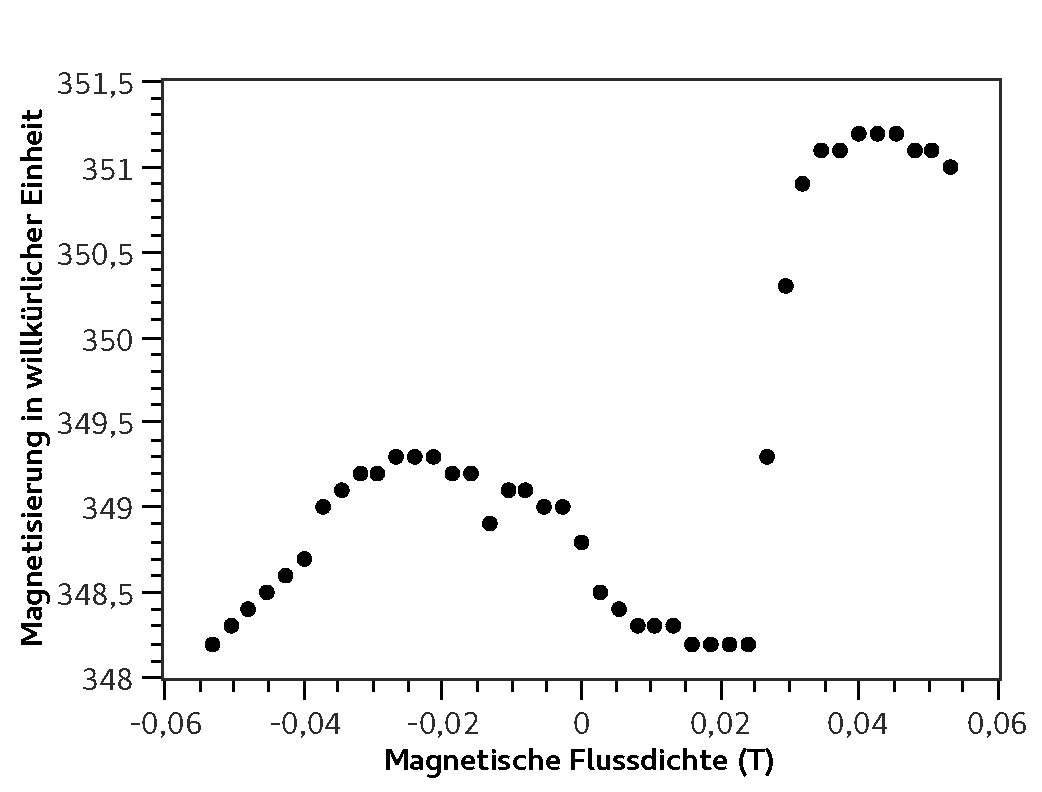
\includegraphics[width=0.65\textwidth]{fig_magn1} %TODO Größe anpassen
		\centering
		\caption{Die Magnetisierung, die durch die Messung der Polarisationsänderung des einfallenden linear polarisierten Lichts gemessen wird, ist gegen die magnetische Flussdichte aufgetragen. Zunächst wurde ein negatives Magnetfeld angelegt. Dieses wurde bis auf Null abgeschwächt und dann ein positives Magnetfeld gesteigert. Die Unsicherheiten sind kleiner als die Symbolgröße.} %TODO hier nur gesenkt und bei anderem dann sagen gesteigert.
		\label{fig_magn1}
		\centering
	\end{figure}

	\begin{figure}[H] %TODO eigentlich "in willkürlichen Einheiten" nicht "in willkürlicher Einheit"
		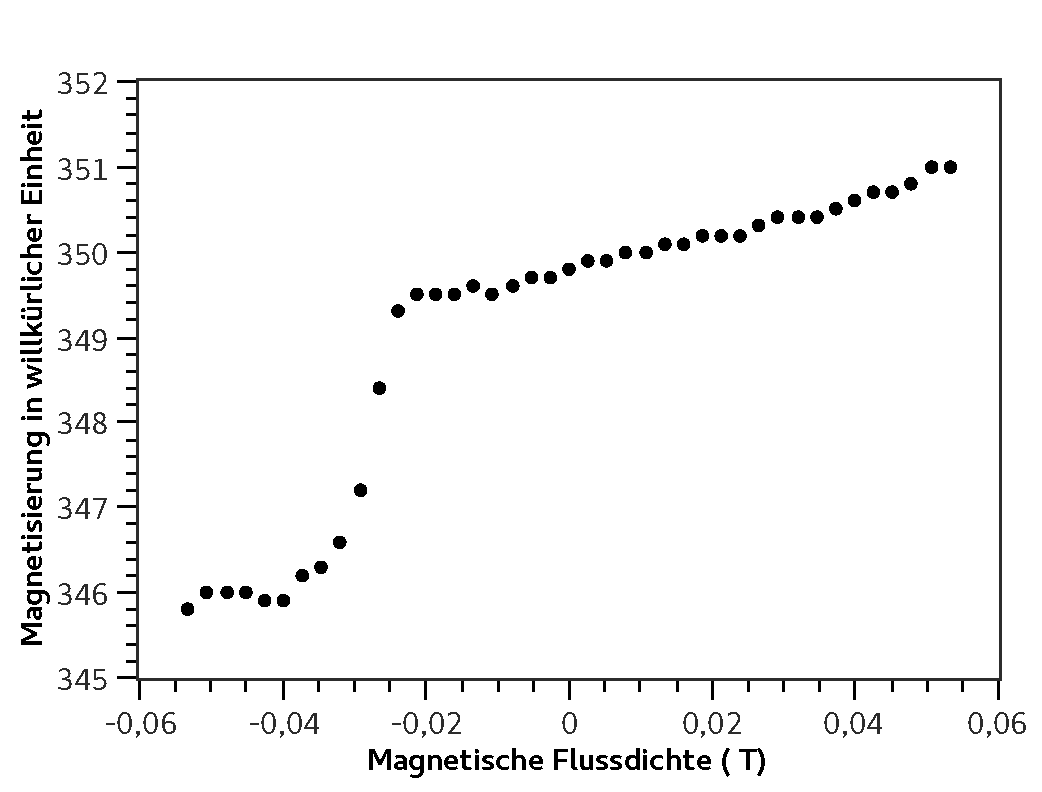
\includegraphics[width=0.65\textwidth]{fig_magn2}
		\centering
		\caption{Die Magnetisierung, die durch die Messung der Polarisationsänderung des einfallenden linear polarisierten Lichts gemessen wird, ist gegen die magnetische Flussdichte aufgetragen. 
		Zunächst ist ein positives Magnetfeld angelegt, dieses wird bis auf Null abgeschwächt und dann in die umgekehrte Richtung erhöht.
		Die Unsicherheiten sind kleiner als die Symbole.} 
		\label{fig_magn2}
		\centering
	\end{figure}
	\subsection{Diskussion}
	%TODO Bezug/Nutzen oder sonst was
	%TODO auch hier die Hypothese wiederholen
	%TODO keine Messwerte hier, nach manchen Menschen, zumindest "direkt" erstellte Diagramme net hier, auch wenn Lesbarkeit-bla

	%TODO wie erwartet ist Spulestrom ~ MAgn FLussdichte
	%TODO fig_magn1, Vorhang bonus licht -> fehler hügel, aber ist nicht Sprunghaft genug
	%TODO Die Sprünge sind bis aufs vorzeichen +- gleich => nice 			
	%TODO Iwas aus der einführung klauen, lul
	
	\section{Schlussfolgerung}
	%TODO Rückgriff auf Hypothese und drittes Nennen dieser
	
	%TODO Quellen zitieren, Websiten mit Zugriffsdatum
	%TODO Verweise auf das Laborbuch (sind erlaubt)
	%TODO Tabelle + Bilder mit Beschriftung
	%\printbibliography
\end{document}
